\section{Hg-Low Linie}
Zuletzt soll die Linie der Hg-Low Lampe untersucht werden. \\
Im Folgenden sind zuerst einmal Darstellungen des Interferogramm der Hg-Low Lampe und 
deren Einhüllende zu sehen:\\
\begin{figure}[h]
    \centering
    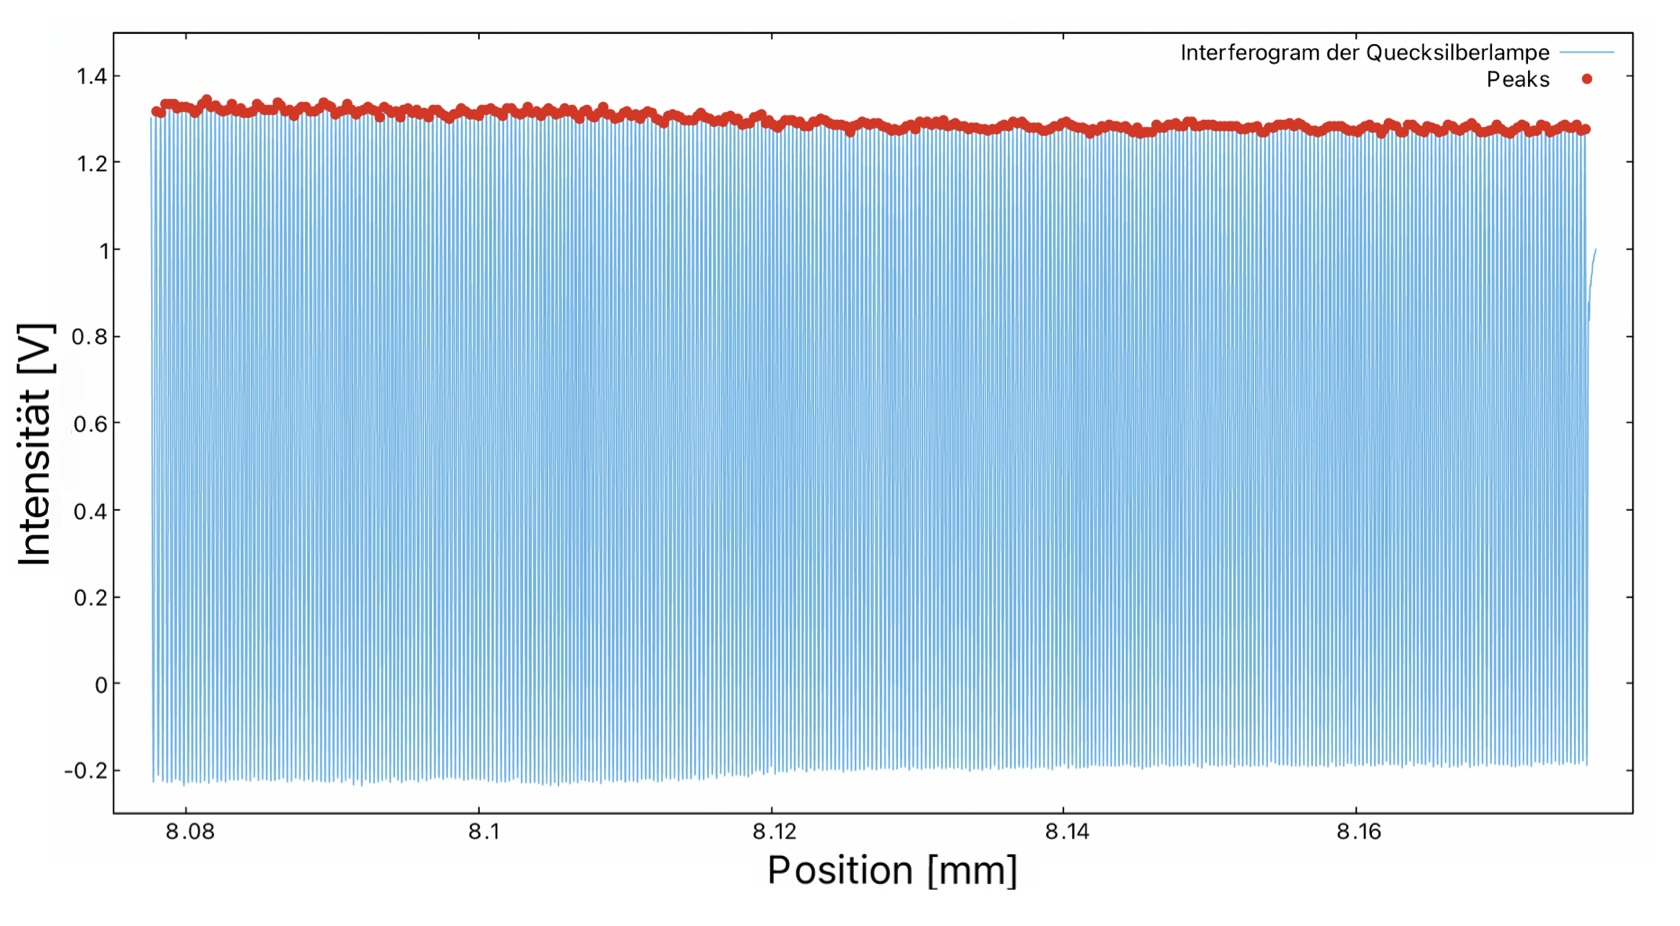
\includegraphics[scale=0.28]{Bilder/Anna/Hg-Low-Interferogram.jpg}
    \caption{Interferogramm der Hg-Linie mit den gekennzeichneten Peaks.}
    \label{fig:IHgLow}
\end{figure}
\begin{figure}[h]
    \centering
    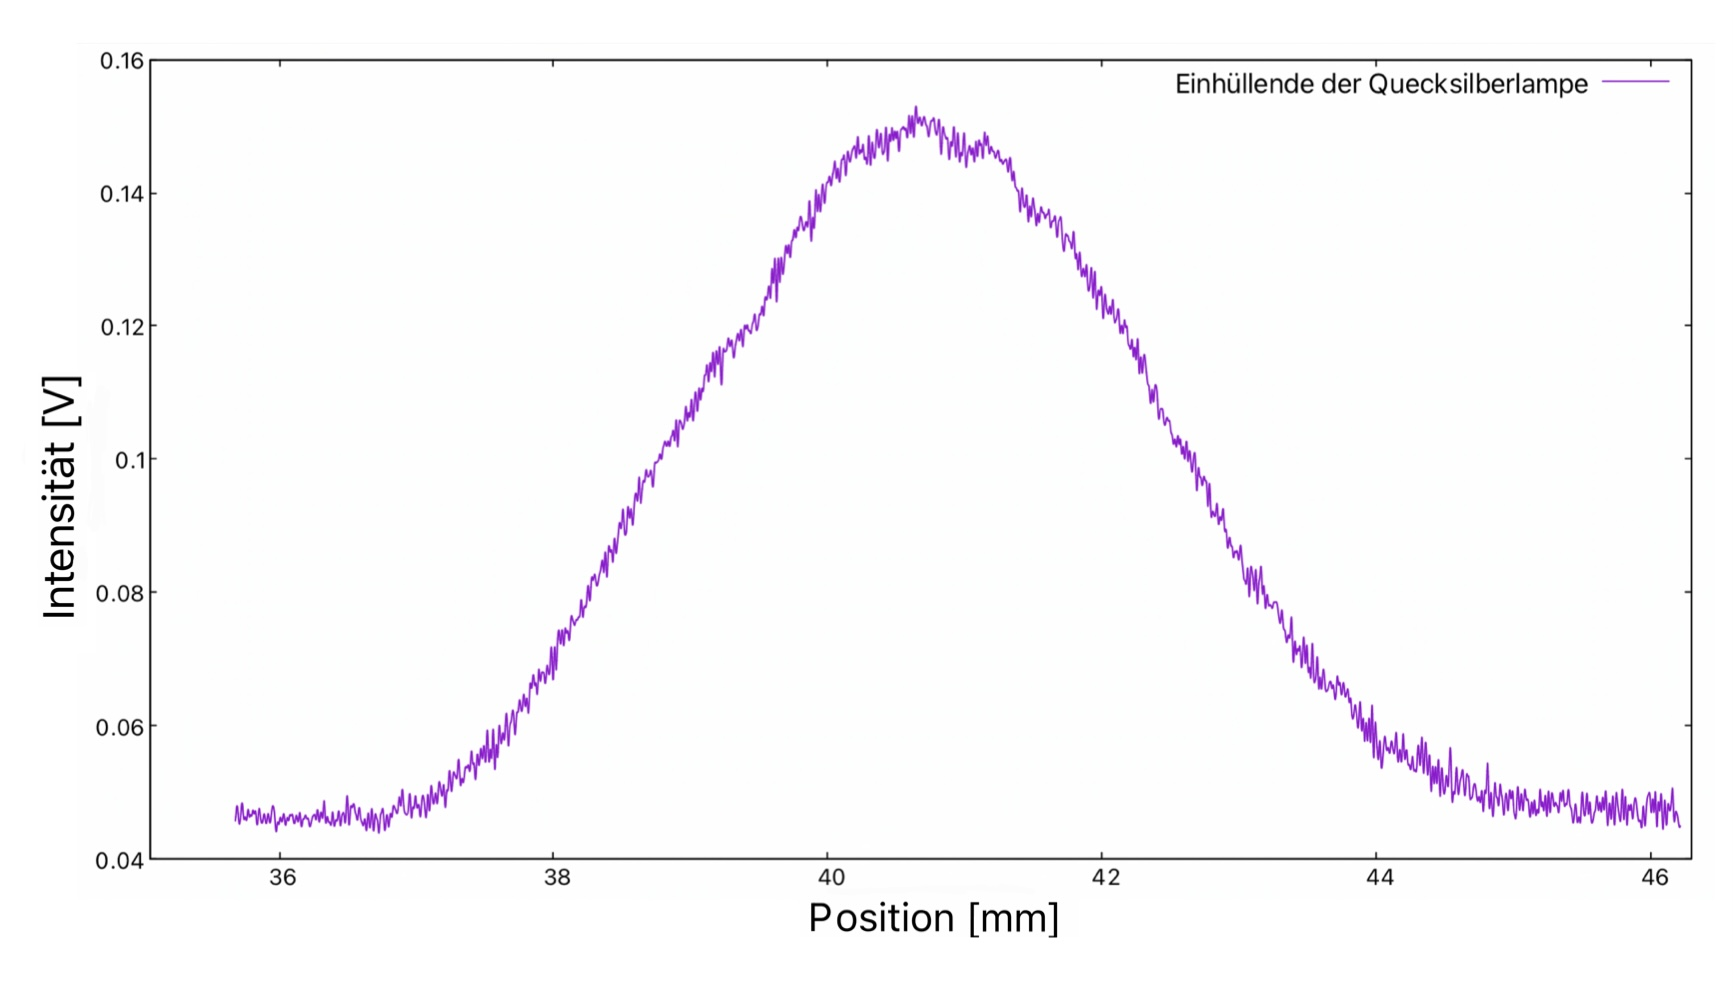
\includegraphics[scale=0.27]{Bilder/Anna/hg-low-ein.jpg}
    \caption{Einhüllende des Interferogramms der Hg-Linie.}
\end{figure}\\
Die Messeinstellungen sind dem Protokoll, im Anhang, zu entnehmen. 
\newpage
\subsection{Wellenlänge}
Die Wellenlänge der Hg-Low Lampe wird analog zur Bestimmung der Wellenlänge der Natrium D-Linie und der Hg-High bestimmt.\\
Auch hier wurden die Peaks des Interferogramms mit einem Python Skript ermittelt, s. Abbildung \ref{fig:PHgLow}. 
Die Anzahl der Maxima der Hg-Low Lampe beläuft sich auf $n_{Hg-Low} = 353$ und die Anzahl der Maxima des Lasers 
auf $n_{Laser} = 305$. Die Wellenlänge des Laser ist $\lambda_L = 632,8\,$nm. Somit folgt für die Wellenlänge
der Hg-Low Linie:
\begin{equation}
    \lambda_{Hg-low} = \frac{n_{Laser}}{n_{Hg-low}} \lambda_L = 546,7535\,\text{nm}
\end{equation}
Analog zur Hg-High Lampe wird auch hier angenommen, dass das Python Skript die Peaks 
bis zu einem Peak genau findet. \\
Somit folgt für den Fehler:
\begin{align}
    s_{\lambda} &= \sqrt{\left( \frac{\partial \lambda_{Hg-low}}{\partial n_{Laser}}\cdot s_{n_{Laser}}\right)^2+ \left(\frac{\partial \lambda_{Hg-low}}{\partial n_{Hg-low}}\cdot s_{n_{Hg-low}}\right)^2}\\
                &= \sqrt{\left(\frac{\lambda_L}{n_{Hg-low}} \cdot s_{n_{Laser}}\right)^2 + \left(\frac{\lambda_L \cdot n_L}{n^2_{Hg-low}} \cdot s_{n_{Hg-low}}\right)^2 }\\
                &= 2,3724\,\text{nm}
\end{align}
Also ist die Wellenlänge der Hg-Low Lampe:
\begin{equation}
    \lambda_{Hg-Low} = (547 \pm 2)\,\text{nm}
\end{equation}\\
Der Literaturwert für Quecksilber ist $\lambda_{Hg-Lit} = 546,1\,$nm \citep[vgl.][]{Zusatzliteratur}.\\
Somit stimmt sowohl die Wellenlänge der Quecksilberhochdrucklampe mit $\lambda_{Hg-High} = (546 \pm 2)\,\text{nm}$, als 
auch die Quecksilberniedrigdrucklampe mit $\lambda_{Hg-Low} = (547 \pm 2)\,\text{nm}$, mit dem Literaturwert überein, v.a.
wenn man den Fehler-Bereich mitberücksichtigt.
\begin{figure}[h]
    \centering
    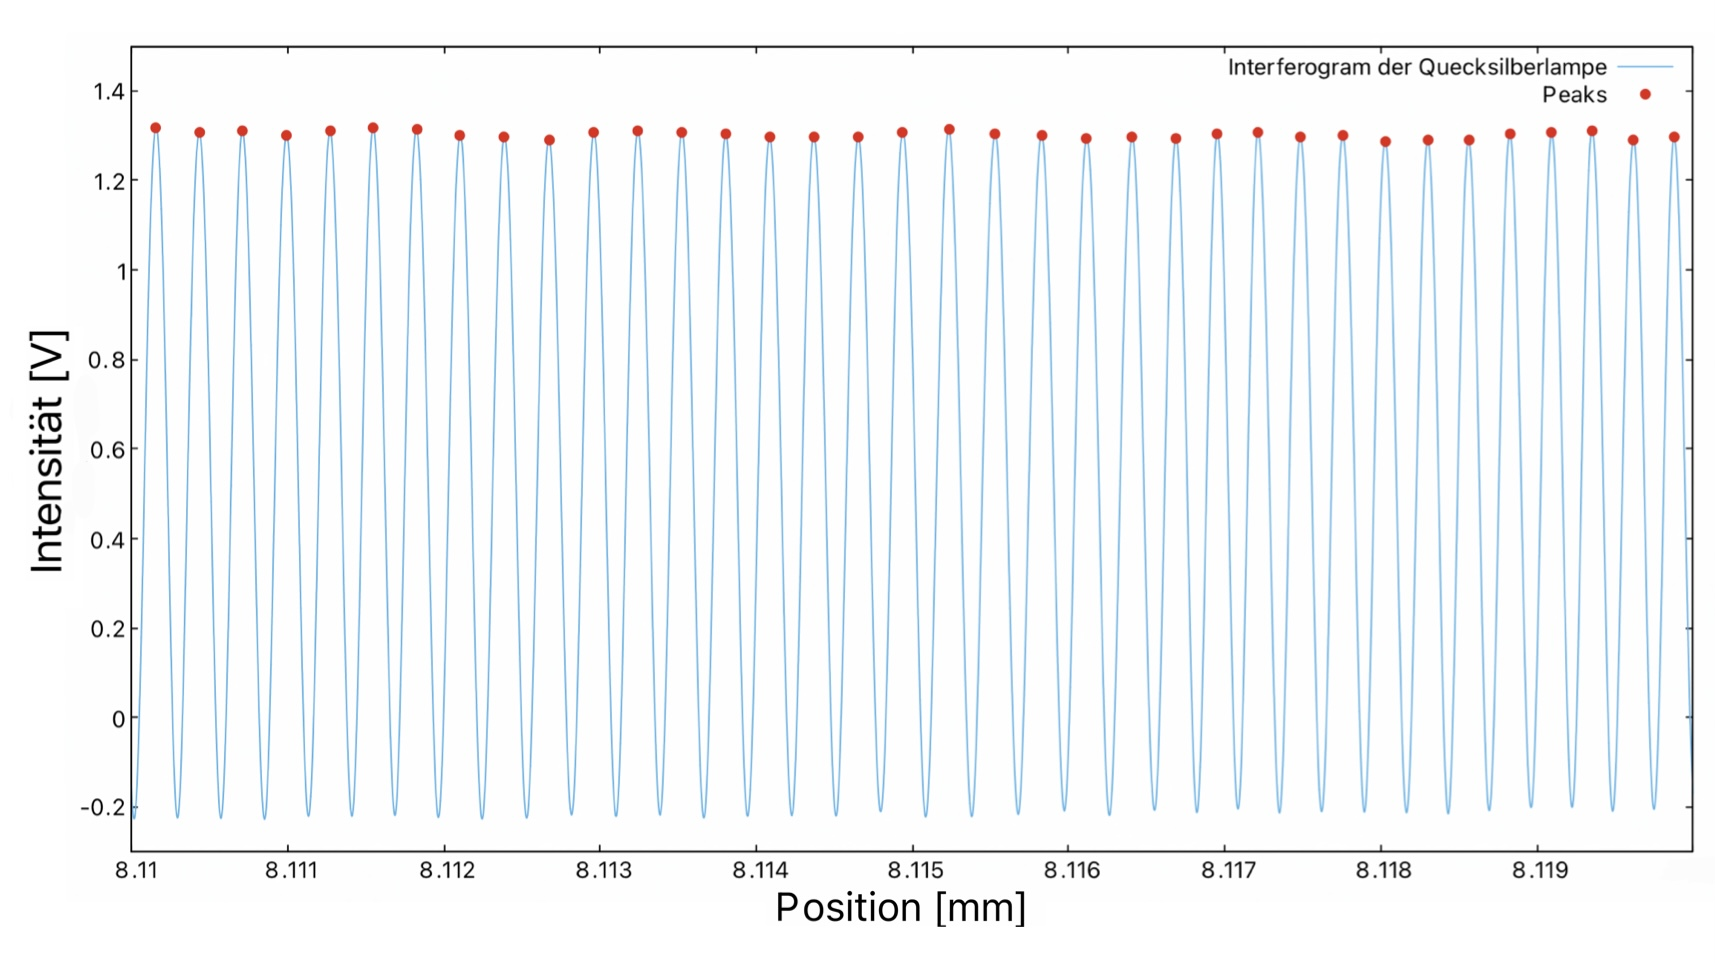
\includegraphics[scale=0.27]{Bilder/Anna/PeaksLow.jpg}
    \caption{Ausschnitt des Interferogramm der Quecksilber Linie und die bestimmten Peaks.}
    \label{fig:PHgLow}
\end{figure}

\newpage
\subsection{Kohärenzlänge}
Als nächstes soll die Kohärenzlänge bestimmt werden. Die Kohärenzlänge ist die Länge der halben Halbwertsbreite der Einhüllenden bei der
die maximale Intensität auf $\frac{1}{e}$ abgefallen ist.\\
Die maximale Intensität der Hg-Low Lampe beträgt:
\begin{align}
 I_0 = (0,1053 \pm 0,0001)\,\text{V}  \\
 \frac{I_0}{e} = (0,03872 \pm 0,0004)\,\text{V} 
\end{align}
Die maximale Intensität wurde aus dem Plot herausgelesen und anschließend der Offset noch abgezogen.\\
Als nächstes muss die Breite der Einhüllenden bestimmt werden bei der die Intensität nur noch $\frac{1}{e}$
beträgt, siehe Abbildung \ref{fig:Hglowe}:
\begin{equation}
    \Delta s_{Hg-low} = 4,2262\,\text{mm}
\end{equation}
Hierbei wird ein Ablesefehler von 0,2 mm angenommen.\\
Nun muss noch der Fehler des Motors 2 berücksichtigt werden, damit man die Kohärenzlänge erhält:
\begin{align}
    L_c = \beta \cdot \frac{\Delta s}{2} = (2,1 \pm 0,2)\,\text{mm}
\end{align}
\begin{figure}[h]
    \centering
    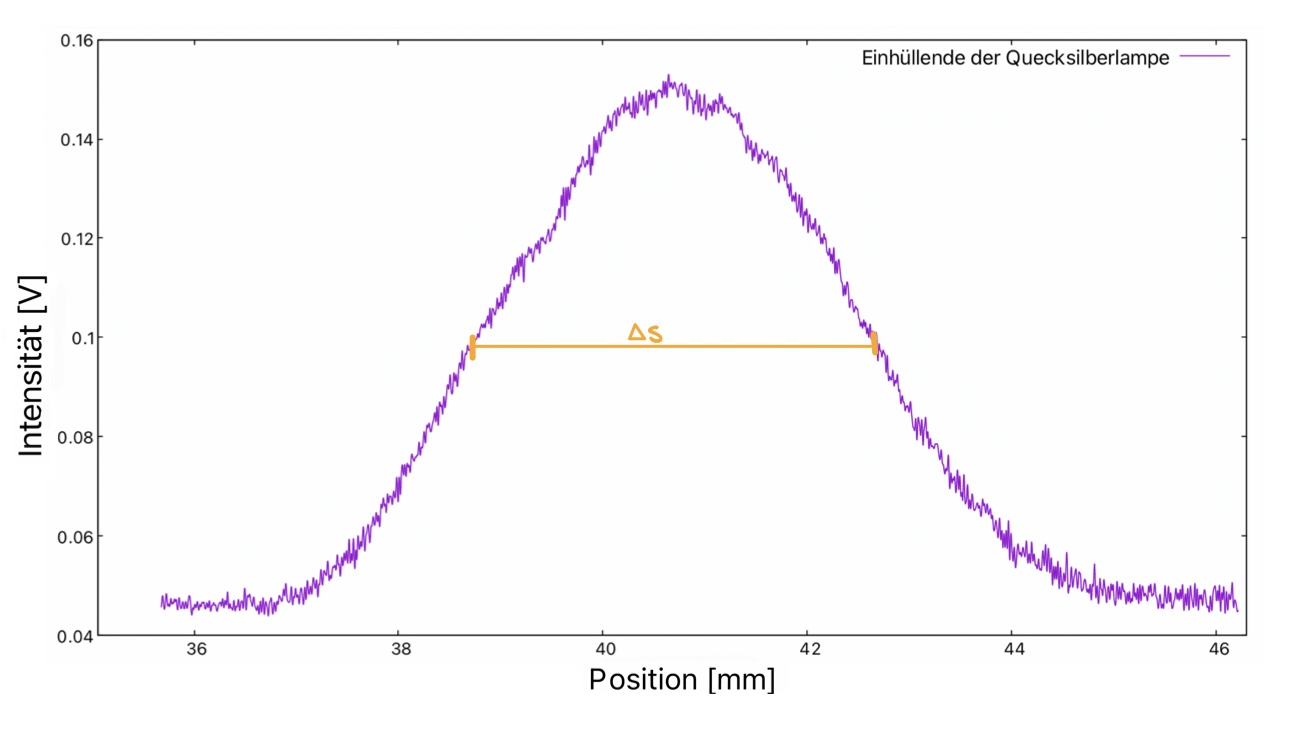
\includegraphics[scale = 0.33]{Bilder/Anna/low1_e.jpg}
    \caption{Einhüllende des Interferogramms der Hg-Linie, zusätzlich wurde noch die Breite, bei der die Intensität nur noch 1/e beträgt, zur Kohärenzlängenbestimmung eingezeichnet.}
    \label{fig:Hglowe}
\end{figure}
\newpage

\subsection{Linienbreite}
Zuletzt soll nun noch die Halbwertsbreite für die Hg-Low Lampe bestimmt werden.\\
Wie man an der Abbildung \ref{fig:Hglowe} erkennen kann, liegt bei der Hg-Low Lampe eine Gaußverteilung vor. 
Somit kann man die Formel für die Halbwertsbreite aus den Fragen zur Vorbereitung (Frage 9) verwenden:
\begin{equation}
    FWHM_{Hg-Low} = \frac{4 \sqrt{ln(2)}}{L_c} = 1,57599 \frac{1}{\text{mm}}
\end{equation}
Die Halbwertsbreite ist in Wellenzahlen angegeben, nun muss sie erneut in Wellenlänge umgerechnet werden, dies 
geschieht wieder mit der in 3.1.2 hergeleiteten Formel:
\begin{equation}
    \Delta \lambda_{Hg-Low} = FWHM \cdot \frac{\lambda^2_{Hg-Low}}{2 \cdot \pi} = \frac{2 \sqrt{ln(2)} \cdot \lambda^2_{Hg-low}}{L_c \cdot \pi} = 0,0800\,\text{nm}
\end{equation}
\begin{align}
    s_{\Delta \lambda_{Hg-low}} &= \sqrt{\left(\frac{\partial \Delta \lambda_{Hg-low}}{\partial L_c} \cdot s_{L_c}\right)^2+\left(\frac{\partial \Delta \lambda_{Hg-low}}{\partial \lambda_{Hg-low}} \cdot s_{\lambda_{Hg-low}}\right)^2} \\
    &= \sqrt{\left(\frac{2 \sqrt{ln(2)} \cdot \lambda^2_{Hg-low}}{L_c^2 \cdot \pi} \cdot s_{L_c}\right)^2+\left(\frac{4 \sqrt{ln(2)}\cdot \lambda_{Hg-low}}{L_c \cdot \pi} \cdot s_{\lambda_{Hg-low}}\right)^2} \\
    & = 0,0071\,\text{nm}
\end{align}
Somit ergibt die Halbwertsbreite der Spektrallinie für die Hg-Low Lampe:
\begin{equation}
    \Delta \lambda_{Hg-Low} = (0,080 \pm 0,007)\,\text{nm}
\end{equation}
Die Einhüllende der Quecksilberniederdrucklampe ist ein Gaußprofil, siehe auch Abbildung \ref{fig:gaussfit}. Das 
heißt allerdings auch, dass diese Linie hauptsächlich durch den Dopplerverbreiterungsmechanismus verbreitert wurde.
\begin{figure}[h]
    \centering
    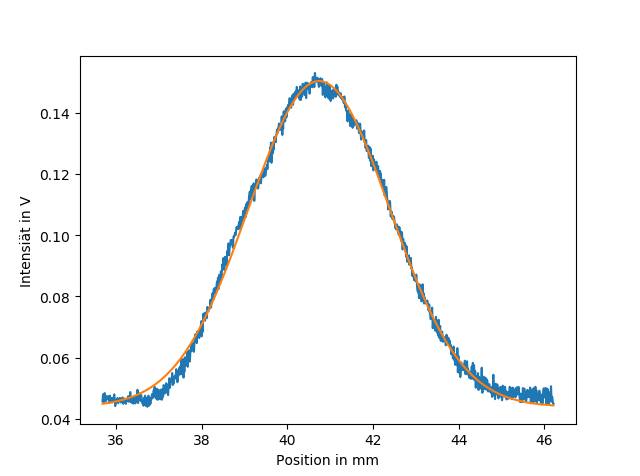
\includegraphics[scale=0.65]{Bilder/Anna/gauss.png}
    \caption{Einhüllende des Interferogramms der Hg-Linie mit Fit-Funktion eines Gaußprofil.}
    \label{fig:gaussfit}
\end{figure}
